\documentclass[letterpaper,twoside,12pt,french]{report}
\usepackage[utf8]{inputenc}
\usepackage[T1]{fontenc}
\usepackage{babel}
\usepackage[top=2.5cm,bottom=2.5cm,left=2.5cm,right=2.5cm,asymmetric]{geometry}
\usepackage{hyperref}
\usepackage{hypcap}
\usepackage{titlesec}
\usepackage{ragged2e}
\usepackage{hyphenat}
\usepackage{berasans}
\usepackage{setspace}
\usepackage{natbib}
\usepackage{float}

\usepackage{abstract}
\renewcommand{\abstractname}{}
\renewcommand{\absnamepos}{empty}
\renewcommand*\familydefault{\sfdefault}
\usepackage[T1]{fontenc}

\usepackage{graphicx}
\graphicspath{{diagrams/}}

\hypersetup{pdftex,colorlinks=true,allcolors=blue}
\newcommand{\reportTitle}{\uppercase{Détection de modèle humain\\Pour application de réalité augumentée}}
\newcommand{\reportAuthors}{Vincent \uppercase{Boiteau-Robert\\BOIV14029409}\\Marc-Antoine \uppercase{Hébert\\HEBM14019401}\\Julien \uppercase{Lemonde\\LEMJ20059208}\\Alexandre \uppercase{Malo\\MALA0702940}}

\newcommand{\abbrItem}[2]{\item[\uppercase{\textbf{#1}} -] #2}
\setlength{\parskip}{1cm plus4mm minus3mm}

\titleformat
{\chapter}
[display]
{\bfseries\Large}
{}
{0ex}
{
    \vspace{0.2ex}
}
{
    \vspace{-0.5ex}
}

\titleformat
{\section}
[display]
{\bfseries\normalsize}
{}
{0ex}
{
    \vspace{-0.5ex}
}
{
    \vspace{-0.5ex}
}

\begin{document}
\setlength{\parindent}{0cm}\setlength{\parskip}{2ex minus 0.2ex}
\pagenumbering{Roman}
\begin{titlepage}
    \begin{center}
        \uppercase{Rapport technique de projet de fin d'études\\Présenté à l'école de technologie supérieure\\Dans le cadre du cours GTI795 Projet de fin d'études en TI}
        \vfill
        \textbf{\reportTitle}
        \vfill
        \reportAuthors
        \vfill
        \uppercase{Département de génie logiciel et TI}
        \vfill
        \textbf{Professeur-superviseur\\Carlos Vazquez}
        \vfill
        \uppercase{Montréal, 25 avril 2018\\Hiver 2018\\Université du Québec}
    \end{center}
\end{titlepage}
\cleardoublepage
\begin{abstract}
    \begin{center}
        \textbf{\uppercase{\Large{Résumé}}}
        \vspace{2ex}
        \\ \textbf{\reportTitle}
        \\ \vspace{1\baselineskip}
        \reportAuthors
        \\ \vspace{1\baselineskip}
        \end{center}
        \par 
        \par
       Le projet consite à détecter un être humain à l'aide d'une caméra 3D afin d'être en mesure 
        d'aller récupérer la texture et la 		profondeur. Pour ensuite convertir l'humain détecté en 
        modèle 3D. Une fois le modèle bâti, le projet consite aussi à intégrer le modèle humain dans 
        une application de réalité augmenté. Celle-ci repose sur framework ARKit de Apple.
        Le tout, encapsuler dans une seule et même application unique. 
        \par
       Ce document contient une introduction sur le sujet ainsi qu'une revue de la documentation utilisé
        pour la réalisation de ce projet. De plus, la méthodologie de travail utilisé et le processus de conception
        y sont documentés. Le tout se termine avec une discussion et une conclusion.
    \vspace{-\baselineskip}
\end{abstract}
\tableofcontents
\listoftables
\listoffigures
\chapter*{\uppercase{Liste des abbréviations}}
\begin{enumerate}
        \abbrItem{ÉTS}{École de Technologie Supérieure}
        \abbrItem{AR}{Augmented Reality ou en français Réalité Augmentée}
        \abbrItem{SDK}{Software Development Kit ou en français Trousse de développement logiciel}
        \abbrItem{API}{Application Programming Interface ou en français Interface de programmation}
        \abbrItem{AV}{audio-vidéo}
\end{enumerate}
\cleardoublepage
\pagenumbering{arabic}
\chapter*{\uppercase{Introduction}}
\addcontentsline{toc}{chapter}{INTRODUCTION}
La performance des caméras des appareils mobiles est en constance croissance depuis quelques
années. Ce qui permet d'envisager l'usage de ces appareils dans des nouveaux domaines d'activités.
Un de ces domaines est la réalité augmentée, où la superposition d'éléments virtuels sur une
capture de l'environnement réel en temps réel. Une démocratisation du développement d'application
utilisant cette technologie s'est faite au cours de l'année précédente, 2017. En effet, la nouvelle
interface de programmation applicative ARKit conçue par Apple offre un environnement de
développement simplifié au développeur d'applications \citep*{StattN2017}. Toutefois, ces technologies
permettent l'interaction avec des modèles générés de façon synthétique. Un défi qui n'a pas encore
de solution reconnue est l'usage de modèles provenant de l'environnement de l'utilisateur dans la
réalité augmentée. Certaines technologies offrent des pistes de solution, mais leur taux d'adoption
et le niveau de compatibilité avec les autres outils de l'environnement de développement Apple est
limité.
\par
Une des technologies les plus intéressantes est le Structure Sensor\citep*{molitchHou01}. Celle-ci
consiste en un périphérique qui doit être attaché à l'appareil. Le périphérique ajoute une caméra
et un senseur 3D. Avec l'usage de la caméra de l'appareil, celui de l'appareil ont peut avoir une
meilleure compréhension de l'environnement 3D. L'outil vient avec une trousse de développement
logiciel permettant de prendre les coordonnées d'un objet sous quatre dimensions, x, y, z et la
couleur. Toutefois cette solution n'est pas très connue et a un nombre de ressources limitées.
\par
Les deux technologies décrites plus haut apportent chacune des possibilités très intéressantes pour
le développement d'application de réalité augmentée. L'usa\hyp{}ge des fonctionnalités d'une dans l'autre
serait très intéressant. Toutefois au moment où l'équipe a débuté le projet, il n'y a pas
d'interface une telle combinaison. Les deux interfaces utilisent la caméra, par contre chacun
utilise un utilitaire différent pour le contrôle de celle-ci. Les deux utilisent des modèles
numériques 3D, mais chacun a choisi une norme différente. En effet, le Structure Sensor permet
l'extraction en Modèle I/O. Alors que le ARKit utilise les modèles de type scène qui est un format
propriétaire à Apple. Le principal défi du projet consistera à la combinaison de plusieurs
interfaces de programmation pour créer un outil fonctionnel.
\par
Comme décrit dans la section précédente, le principal objectif du projet est la création d'une
interface entre deux technologies mobiles, soit un périphérique d'acquisition de modèle 3D, le
Structure Sensor et la trousse de développement de réalité augmentée d'Apple. Autrement dit,
l'équipe s'attend en fin de session d'avoir produit une application mobile permettant la prise
de modèle à l'aide du senseur. L'application permettra d'ajouter un modèle extrait sur une surface
plane. L'application permet cette chaîne d'action avec une expérience utilisateur agréable et
naturelle à l'utilisateur.
\par
L'application décrite ci-haut représente les attentes pessimistes par rapport aux résultats finaux.
Toutefois, une telle application apporte un éventail de possibilités sur la manipulation de
l'environnement augmentée. Par exemple, une des retombées envisageables et
commercialisables est la numérisation de catalogue de magasin comme Ikea. L'usager peut
donc ajouter un item dans une pièce de sa maison. Si plusieurs couleurs sont disponibles pour
un modèle, chacune des variantes sera disponible à la modélisation.
\par
Une autre ouverture technologique, qu'une telle application apporterait, est dans un contexte
d'animation 3D. En effet, la création d'un modèle permettrait l'ajout d'un squelette dans celui-ci.
Une fois le squelette créé l'animation du modèle pourrait être fait. Cette possibilité est
particulièrement intéressante pour l'équipe responsable du projet. Dans l'éventualité où la vision
de base du projet sera complétée avant la fin de la session d'Hiver 2018, l'équipe compte se
concentrer sur la création de ce squelette et possiblement la manipulation de celui-ci. La création
de positionnement clé des noeuds du squelette pourra être enregistrée afin de permettre l'animation.
L'animation libre est un trop grand défi étant donné les contraintes de temps.
\par
L'objectif principal semble réaliste pour l'équipe de développement étant donné les interfaces déjà
présentes pour chacune des technologies. Toutefois, le défi reste important étant donné le manque de
cohérence entre les différentes technologies. Le manque de documentation et de support pour le
Structure Sensor risque d'amener un ensemble de défi supplémentaire.
\par
Par contre, l'équipe de développement considère le temps disponible à la résolution d'un tel enjeu
adéquat. L'expérience en recherche d'information et apprentissage autonome acquise au cours des
formations et stages des membres de l'équipe laisse envisager un succès.
\par
Pour ce qui est en la complétion des objectifs accessoire, les limitations de temps rendent
l'estimation de succès plus difficile. Par contre, il est clair que la réalisation de ceux est
apporterait un plus considérable à l'expérience de chacun des membres. La motivation de l'équipe
face à l'enjeu améliore les probabilités de terminer ces objectifs.
\par
Ce rapport consiste donc en un suivi des étapes qui permettront de valider ou invalider les
hypothèses décrites si haut. Afin de résoudre un tel défi, l'équipe a dû se fier sur les
documentations disponibles en lien avec les technologies ciblées. Un résumé de celles qui ont été
utiles à la résolution du problème sera présenté.
\par
Par la suite, une présentation de la méthodologie utilisée par l'équipe sera décrite. Les étapes
ayant permis la conception de la solution seront par la suite présentées. Une analyse sur le produit
obtenue sera explorée. Afin de clore le projet, les possibilités que la solution apporte à un groupe voulant poursuivre ou
implémenter un projet semblable seront expliquées. L'équipe fera s'est recommandation en fonction
de l'expérience acquise lors du développement.
\chapter*{\uppercase{Revue de la documentation}}
\addcontentsline{toc}{chapter}{REVUE DE LA DOCUMENTATION}
Afin de réaliser le projet, l'équipe de développement a dû faire des recherches préliminaires. Les
technologies utilisées n'étaient pas maitrisées par l'équipe au démarrage du projet. Donc, les
recueils de documentation et les projets exemples présents sur internet ont été une bonne source
d'information.
\par
Cette section présentera donc ces ressources pour les grandes parties du projet,
soit le périphérique Structure Sensor, la trousse de développement logiciel de réalité augmentée de
Apple et la gestion de projet.
\section*{Structure Sensor}
\addcontentsline{toc}{section}{Structure Sensor}
Occipital, la compagnie propriétaire du périphérique, publie régulièrement une version de leur
trousse de développement logiciel exposant des interfaces de programmation. La dernière version
publiée par la compagnie est la version 0.7.1 en février 2018. \citep*{occipitalsdk} La version du
SDK étant inférieure à 1.0.0, on comprend que la première version complète est encore en
développement.
\par
Dans l'état actuel, le SDK fournit quand même une liste d'interface disponible dans deux fichiers,
Structure et StructureSLAM. Le premier est composé des différentes interfaces de contrôle du
périphérique. Alors que le deuxième est un regroupement des classes permettant le contrôle des
mailles en position tridimensionnelles et les textures de ceux-ci.
\par
Ces interfaces seront la base de la conception du module de prise de modèle grâce au périphérique.
Les tâches de chacune des interfaces ont été identifiées lors de la lecture du code des entêtes
des interfaces en Objective-C. L'équipe a produit un diagramme de classe afin d'améliorer la
compréhension des responsabilités de chacune des interfaces et les relations entre celles-ci.
Celui-ci est présenté à la page suivante.

\begin{figure}[H]
    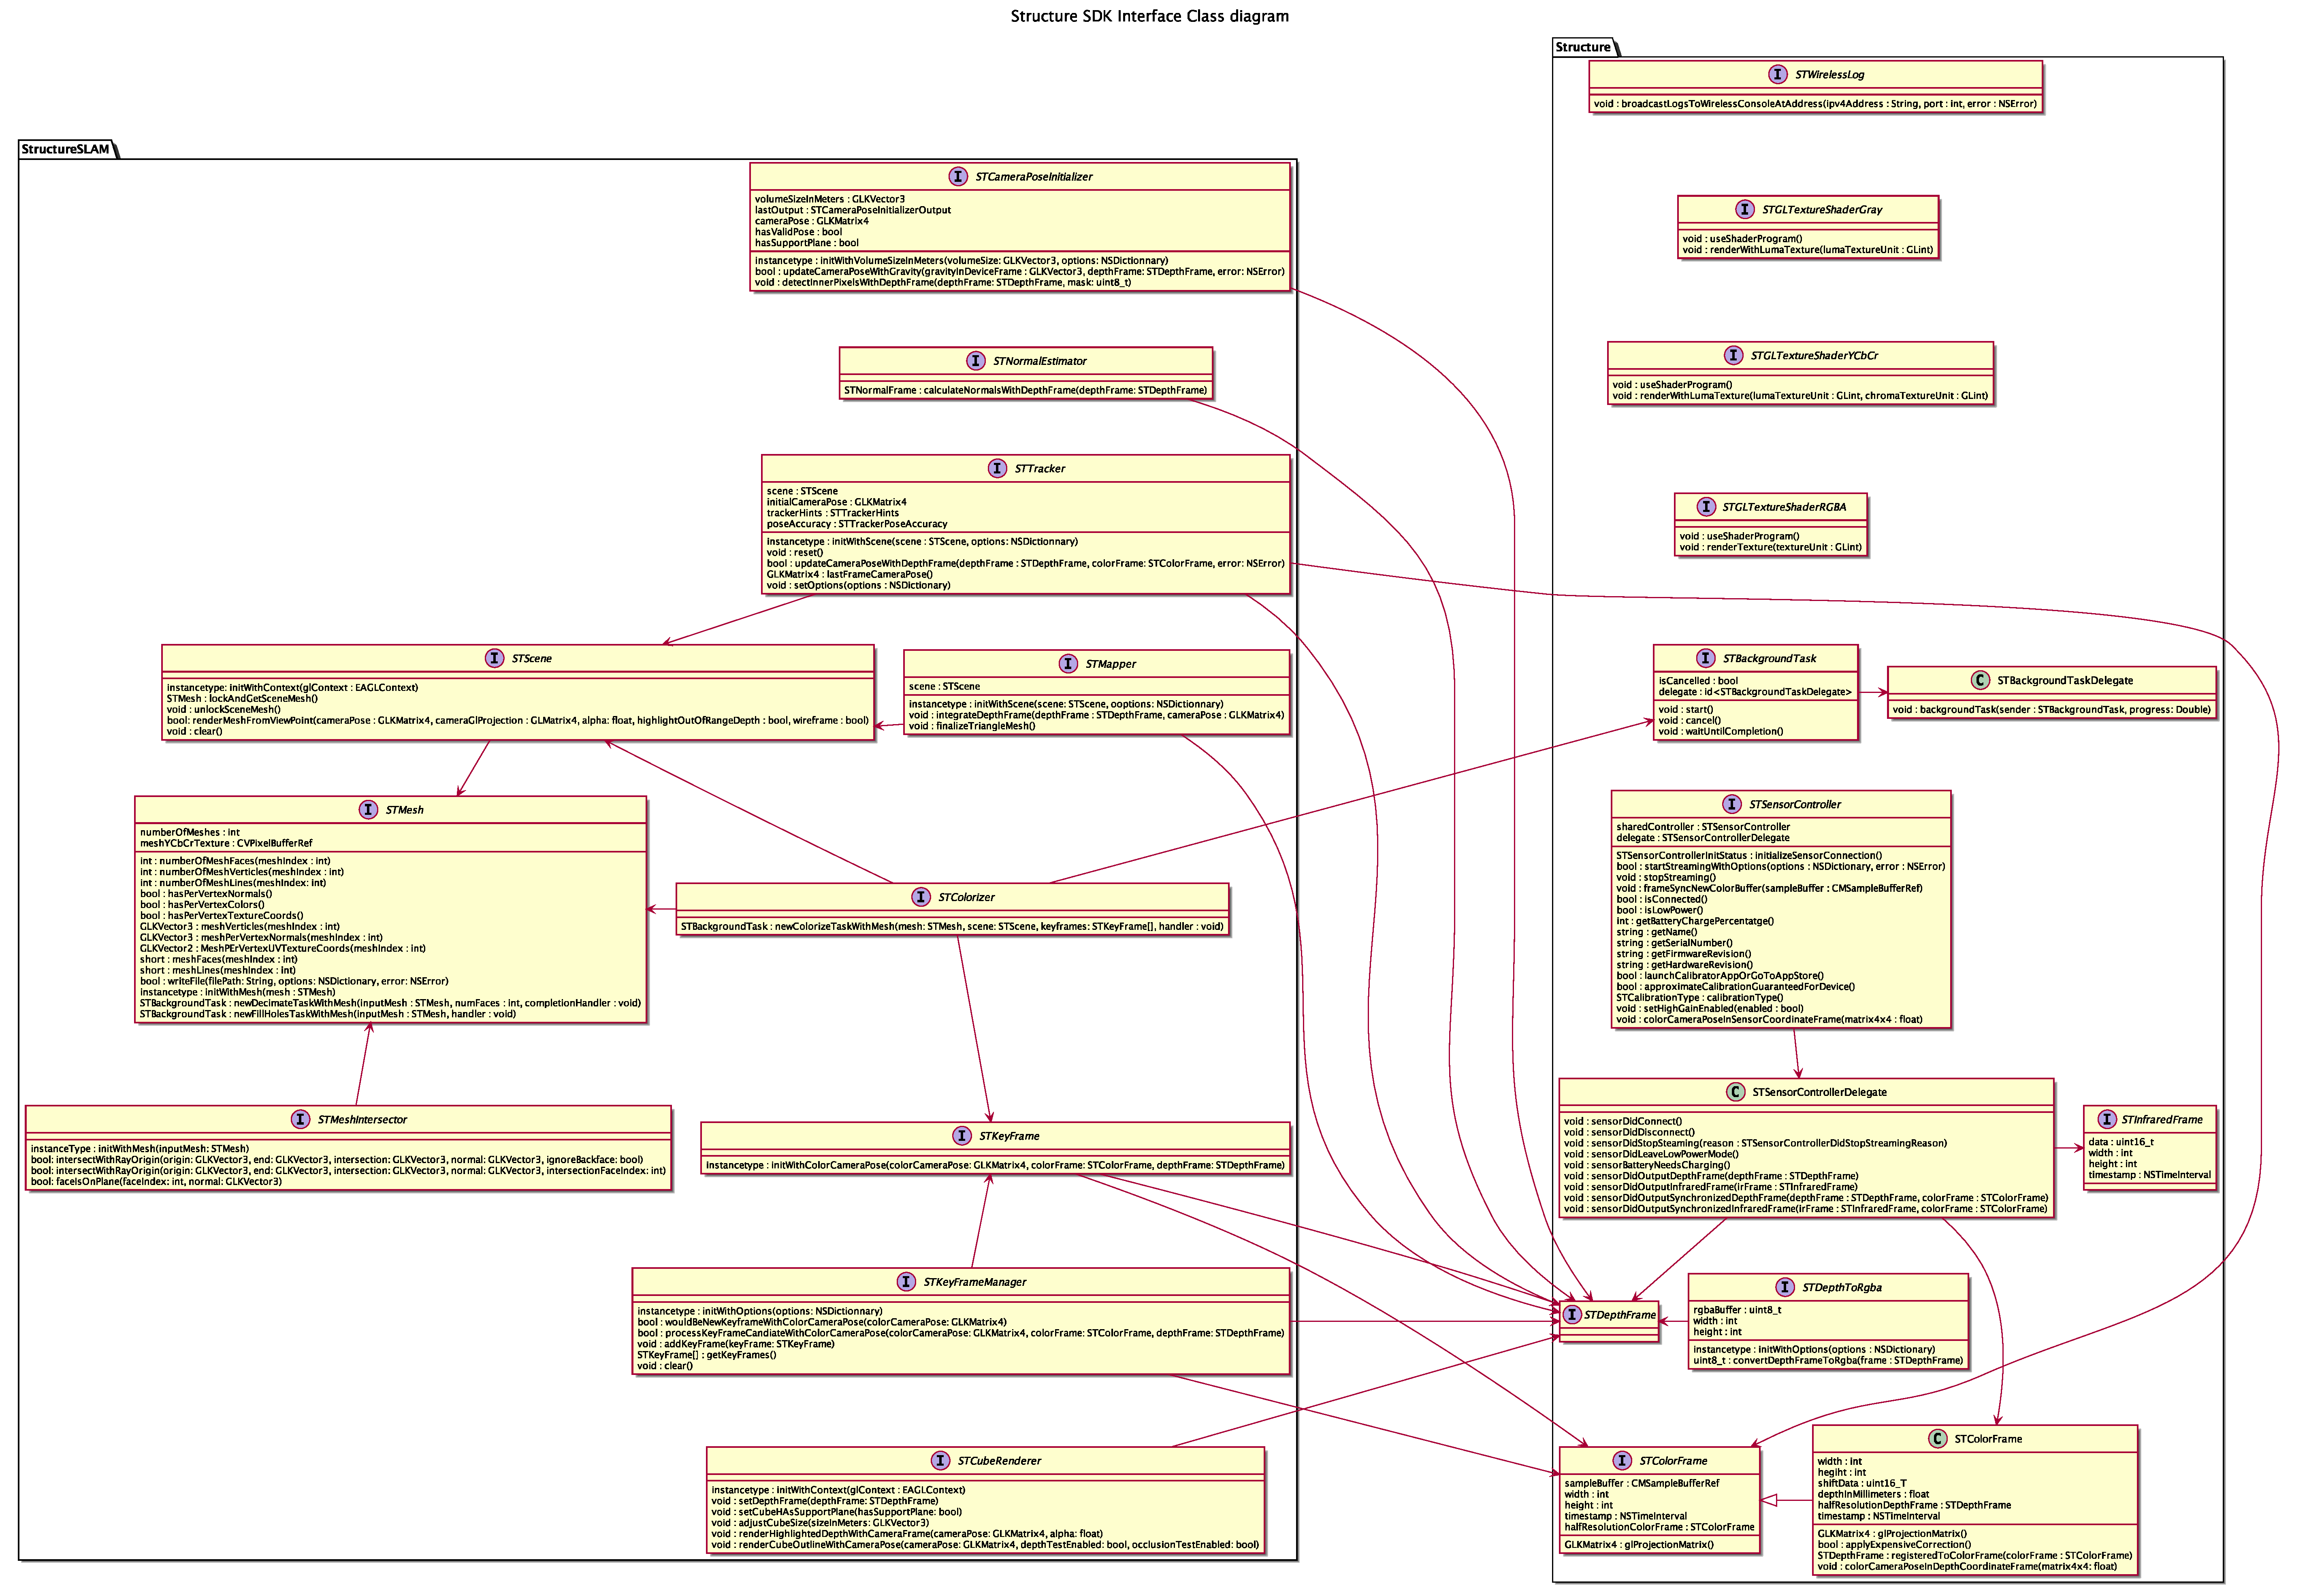
\includegraphics[width=\textwidth]{StructureClassDiagram.eps}
\centering
    \caption{Diagramme de classes du Structure Sensor SDK}
\end{figure}

Dans le diagramme, on constate que plusieurs patrons de conception ont été utilisés et exposés dans
l'interface. La classe STSensorControllerDelegate servira de point d'ancrage entre notre
application et le Structure Sensor. Cette interface permet donc de réduire les communications ou 
les recherches d'informations dans la logique d'affaires. La plupart de l'usage du SDK dans
l'application devra être fait par cette classe. \citep*{bpse01}
\par
Le Structure Sensor utilise les DepthFrame et ColorFrame pour comprendre l'environnement dans lequel
il est utilisé. Ces concepts ont été introduits par Kinect un des premiers Senseurs 3D ayant connu
un succès commercial étant donné sont intégration dans l'environnement Xbox 360 de Microsoft.
\citep*{microsoft01}
\par
Le Structure SDK contient aussi plusieurs exemples d'application afin de guider les développeurs dans
le développement de leurs applications. Le plus intéressant pour l'objectif du projet est le
Scanneur. Celui-ci permet de convertir un objet dans l'espace de test en un modèle 3D et l'envoyer
par courriel. D'autres fonctions incluses dans cet exemple sont la colorisation du modèle et les
différentes options de capture. L'espace de capture est aussi indiqué par un cube et un plan
utilisant les couleurs pour indiquer les objets qui peuvent être capturés.
\par
Les principales sections du SDK utilisé dans cet exemple sont le STStructureSensorDelegate pour le
contrôle du périphérique. Les STDepthFrames et les STColorFrames ou en français les grilles de
profondeurs et les grilles de couleurs permettant de créer le modèle STMesh. Une fois le modèle
scanner en maille celui-ci est présenté dans le MeshViewController grâce au rendu de maille,
STMeshRenderer. Le langage de programmation utilisé dans la globalité du SDK est le Objective-C.
\par
Dans le but d'utiliser des technologies qui sont à jour avec les pratiques de l'industrie, l'équipe
de développement souhaite utiliser le nouveau langage de programmation Swift. Celui-ci est le
nouveau langage proposé par Apple pour le développement mobile. Le langage est déjà à sa quatrième
version majeure et a pour but de simplifier la syntaxe qui était auparavant utilisée soit le
Objective-C. \citep*{swift01} Un membre de la communauté de développeur Structure à produit un
port de l'exemple de Scanneur en Swift 2. L'équipe devra donc faire les changements nécessaires à
cette version pour la compiler avec la version 4. \citep*{structureScannerSwift}
\par
L'exemple de scanneur qui sera utilisé comme base du module de scan utilise plusieurs autres APIs
par Apple. Ces APIs sont documentées sur le site de Apple dans la section pour développeurs.
\citep*{appleDev} L'équipe utilisera donc cette ressource en ligne pour accomplir la tâche.
\chapter*{\uppercase{Méthodologie de travail}}
\addcontentsline{toc}{chapter}{MÉTHODOLOGIE DE TRAVAIL}
La démarche entreprise par l’équipe de développement pour compléter le projet a été basé sur la
combinaison des acquis obtenus dans les projets résolus en stage et au cours du processus
universitaire. Toutefois la nature du projet de fin d’études comprend des contraintes et conditions
qui ont dû être prises en compte.
\section*{Planification}
\addcontentsline{toc}{section}{Planification}
Tout d’abord, aucun des membres de l’équipe n'avait des connaissances dans les technologies qui
devaient être traitées dans les projets. Il a donc été nécessaire de faire une recherche
préliminaire afin de gagner une compréhension nécessaire à la planification du projet. La
recherche à permis de répondre à des enjeux surs qu’elles étaient les principales parties du projet?
Quelles technologies étaient incluses implicitement au ARKit et Structure Sensor? Quel environnement
de développement devait être utilisé? Est-ce que les objectifs étaient réalistes dans les
contraintes de temps et de ressources?
\par
Suite à cette recherche, le projet ayant été jugé comme réalisable a été séparé en plusieurs modules.
C’est à dire des parties du projet qui peuvent être développées indépendamment et être assignées à
différents étudiants. Ayant conscience de la possibilité de bloquants au cours du développement
cette technique permet de ne pas limiter l’avancement du projet complet, dès qu’il y a un problème.
Les différents modules identifiés sont: le développement du scanneur avec le Structure Sensor, le
développement de l’environnement AR et le développement du squelette dans le modèle humain. Le
dernier module a été identifié comme accessoire étant donné l’importance de l’enjeu. De plus, le
développement des deux premiers modules et leur combinaison est déjà importante en taille et
complexité.
\par
Une fois les deux modules principaux identifiés, une séparation de l'équipe de développement a été
faite. La séparation visait à permettre à chacun de se concentrer sur un type d'enjeu et de
diminuer la grosseur des défis. De plus, cette méthode a permis de répondre à des contraintes qui
entourait le projet et les technologies disponibles. En effet, un seul périphérique Structure
Sensor était disponible. De plus, trois développeurs sur quatre avaient accès à un appareil Apple
mobile.
\par
Une fois les sous-équipes identifiées, celles-ci ont dû séparer et lister les tâches à
accomplir, les ressources documentaires disponibles autour de leur technologie et lister les
risques que leurs technologies impliquaient. Ces informations ont été ajoutées au plan de projet avec
la description du projet et la mise en situation. Les tâches ont été par la suite séparées en trois
jalons de développement.
\par
Pour le module de Structure Sensor, les trois jalons consiste en le transfert du projet Scanneur de
Swift 2 à Swift 4 pour le premier. Pour le second, la cible était l'intégration dans la structure 
de l'application AR et le transfert du modèle dans l'application. Le troisième consistait en la 
conception d'une interface visuelle adéquate et une possibilité de faire un début de squelette sur
le modèle humain.
\par
Pour le module de réalité augmentée, les trois jalons sont la sélection d'un modèle dans une liste,
l'ajout dans la scène et la suppression de celui-ci pour le premier. Pour le second, la modification
à l'aide des gestures classiques d'éditions d'objets sur un appareil mobiles. Pour le troisième, la
conception de l'interface visuelle et une possibilité de contrôle des poses du squelette humain.
\section*{Jalon}
\addcontentsline{toc}{section}{Jalon}
Chaque jalon représentant une partie du travail à faire contiendra toujours un certain nombre 
commun de regroupements de tâches. Pour commencer, avant d'entreprendre toute forme de travail, des
recherches doivent être faites. Les éléments concernant les différentes méthodes de réalisation d'une
tâche et les avantages et désavantages de chacune de celles-ci doivent être identifiés.
\par
Par la suite, une solution doit être sélectionnée en comparant les avantages et désavantages.
Le contexte de développement de l'application doit être aussi pris en cause. Une fois la solution
choisie, l'adaptation de la conception de la solution doit être faite pour le cadre du projet. Si
la solution s'intègre au sein d'une autre solution, les documents de conceptions de la solution
parentes sont adaptés. La conception est donc souvent itérative à travers les jalons et les
tâches.
\par
Par la suite, la solution est intégrée dans l'application à l'aide de l'éditeur spécialisé XCode.
La compilation et la mise en marche est testé sur un appareil mobile Apple au fur à mesure du
développement afin d'éviter les mauvaises surprises en fin de jalon. Une fois une tâche terminée,
le cas d'utilisations principal de l'application est testé pour s'assurer qu'aucune autre
fonctionnalité n'a été brisée.
\par
Le jalon est par la suite terminé avec une revue du travail fait et avec une présentation préparée par
l'équipe pour le superviseur du projet. Dans ces revues on discute du travail fait, des bloquants
et du travail à faire. Les artéfacts de conception et documents de projets doivent aussi être mis à
jour.
\section*{Clôture}
\addcontentsline{toc}{section}{Clôture}
Le développement applicatif terminer, certaines tâches doivent être faites afin de clore le projet.
Parmi celles-ci est la revue des résultats obtenue par l'équipe de développement. Cette tâche a pour
but d'évaluer l'état de l'application par rapport au résultat qui était attendu en début de projet.
Dans le cas de différences entre les attentes et le produit final, un bilan de justification  doit
être tenu.
\par
Par la suite, l'équipe devra lister ces recommandations qui pourraient servir à une autre équipe voulant
poursuivre le projet. Le contexte de projet de fin d'études permet en effet la poursuite d'un tel
projet. Alors un transfert de connaissance doit être préparé afin de limiter les frictions des
futures parties prenantes au projet. Les deux dernières tâches permettront la préparation de la
présentation qui sera faite en fin de projet devant d'autres étudiants finissants.
\chapter*{\uppercase{Processus de conception}}
\addcontentsline{toc}{chapter}{PROCESSUS DE CONCEPTION}
La démarche décrite dans la dernière section permettra de structurer les tâches de conception
exécutées par chaque membre de l'équipe. Ainsi qu'avec les informations obtenus dans la revue
documentaire, une solution à l'enjeu soulevé en début de projet a été conçu. Les besoins comblées,
le fonctionnement de la solution, les différentes solutions explorées et la solution retenue et
prototypée seront présentés.
\par
Les responsabilités que la solution développée devra couvrir consiste en: La prise de modèle dans
l'environnement réel, la présentation de ces modèles dans l'environnement réel pris par la caméra,
la compréhension des coordonnées de l'environnement capturé, la modifications du modèle et la
reconnaissance des mouvements de l'appareil. La technologie Structure Sensor peut répondre au
responsabilité de prise de modèle dans l'environnement et compréhension des coordonées de l'
environnement réel. Par contre, les autres responsabilités devront être résolues par d'autres
moyens.
\par
Deux possibilités se sont révélées comme intéressantes lors des recherches. La première consistant
en le développement d'une solution personnalisée permettant la gestion du modèle déjà scanner.
Cette gestion devrait permettre l'ajout du modèle dans un environnements contrôlées à l'aide des
coordonées acquise grâche au Structure Sensor. Une fois ajouté dans l'environnement le modèle doit 
pouvoir être déplacer, mis à l'échelle et être pivoter. Ce modèle devra pouvoir être supprimer de
l'environnement. Toutes ces différentes tâches demandent donc un cadre de développement permettant
la transformation des données provenant des périphérique de capture en scène tri-dimensionnelle
avec lesquels les développeurs intéragissent.
\chapter*{\uppercase{Discussion}}
\addcontentsline{toc}{chapter}{DISCUSSION}
discussion text
\chapter*{\uppercase{Conclusion}}
\addcontentsline{toc}{chapter}{CONCLUSION}
conclusion text
\newpage
\begin{spacing}{1}
    \nocite{*}
    \bibliographystyle{bibETS}
    \addcontentsline{toc}{chapter}{BIBLIOGRAPHIE}

    \bibliography{biblio_fr}
\end{spacing}
\end{document}
